\chapter{KIẾN THỨC NỀN TẢNG}\label{chapter:knowledge}
\section{Phân biệt ảnh y khoa và ảnh kỹ thuật số thông thường}

\subsection{Định nghĩa và phân loại ảnh kỹ thuật số}
Ảnh kỹ thuật số là hình ảnh bao gồm các điểm ảnh, điểm ảnh này được gọi là pixel. Mỗi pixel có số lượng biểu diễn số hữu hạn, riêng biệt cho cường độ và mức xám của nó, là đầu ra từ các hàm hai chiều của nó được cung cấp dưới dạng đầu vào bởi tọa độ không gian được biểu thị bằng x, y trên trục x và trục y tương ứng. Tùy thuộc vào việc độ phân giải hình ảnh được cố định, nó có thể thuộc loại vectơ hoặc raster.

\subsubsection{Ảnh kỹ thuật số được chia làm hai loại}
\paragraph{Ảnh raster}là một tập hợp hữu hạn các giá trị kỹ thuật số, được gọi là phần tử ảnh hay pixel. Hình ảnh kỹ thuật số chứa một số lượng hàng và cột cố định. Pixel là thành phần riêng lẻ nhỏ nhất trong ảnh, giữ các giá trị đại diện cho độ sáng của một màu nhất định tại một điểm cụ thể. Thông thường, các pixel được lưu trữ trong bộ nhớ máy tính dưới dạng bản đồ raster, là một mảng hai chiều các số nguyên.
\vspace{-0.7cm}
\paragraph{Ảnh vector}là ảnh được tạo bằng kỹ thuật sử dụng các tọa độ trong mặt phẳng 2 chiều đề biểu diễn hình ảnh. Các tọa độ này sẽ góp phần tạo nên các đường và các đường này còn có thể có các thuộc tính như màu nét, hình dạng, độ dày,...
\newpage
\begin{figure}[H]
    \centering
    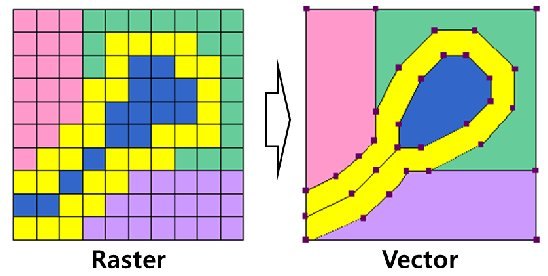
\includegraphics[scale=1.2]{images/medicine/img8.jpg}
    \caption{So sánh ảnh raster và ảnh vector \cite{WinNT2}.}
\end{figure}

\noindent Một ví dụ về đọc và hiển thị ảnh raster bằng python sử dụng opencv.
\vspace{-0.4cm}
\begin{minted}[frame=single,framesep=3pt]{python}
import cv2
import matplotlib.pyplot as plt
img = cv2.imread('img1.png')
\end{minted} 
\vspace{-0.4cm}
Biến img lưu trữ hình ảnh img1.png là một mảng nhiều chiều, muốn hiển thị số chiều của biến img ta chạy lệnh sau:
\vspace{-0.4cm}
\begin{minted}[frame=single,framesep=3pt]{python}
img.shape
=> Output: (384, 430, 3)
\end{minted} 
\vspace{-0.4cm}
Số 384 là chiều rộng của ảnh, số 430 là chiều dài của ảnh, số 3 số là kênh màu  của ảnh.
Để hiển thị hình ảnh dưới dạng mảng nhiều chiều, ta chạy dòng lệnh sau
\vspace{-0.4cm}
\begin{minted}[frame=single,framesep=3pt]{python}
img
array([[[255, 255, 255],
        [255, 255, 255],
        ...,
        [255, 255, 255],
        [255, 255, 255]],
        ...,
        [255, 255, 255],
        [255, 255, 255]]], dtype=uint8)
\end{minted} 
\vspace{-0.4cm}
Để hiển thị hình ảnh, ta chạy những dòng lệnh sau:
\vspace{-0.3cm}
\begin{minted}[frame=single,framesep=3pt]{python}
plt.imshow(cv2.cvtColor(img, cv2.COLOR_BGR2RGB))
plt.show()
\end{minted} 
\vspace{-0.4cm}

\begin{figure}[H]
    \centering
    
\includegraphics[width=8cm]{images/medicine/img10.jpg}
    \caption{Một hình ảnh raster (Nguồn: internet)}
\end{figure}

\subsection{Định nghĩa và phân loại ảnh y khoa}
Ảnh y khoa là kỹ thuật và quy trình tạo hình ảnh trực quan về bên trong của cơ thể để phân tích lâm sàng và can thiệp y tế, cũng như biểu thị trực quan chức năng của một số cơ quan hoặc mô sinh lý học. Hình ảnh y khoa nhằm tìm kiếm các cấu trúc bên trong được che giấu bởi da và xương cũng như chẩn đoán và điều trị bệnh. Hình ảnh y khoa cũng thiết lập một cơ sở dữ liệu giải phẫu học và sinh lý học bình thường để phục vụ việc xác định các bất thường trong mô sinh học. Mặc dù hình ảnh của các cơ quan và mô bị loại bỏ có thể được thực hiện vì lý do y tế, các thủ tục như vậy thường được coi là một phần của bệnh lý thay vì hình ảnh y khoa.

\subsubsection{Các loại ảnh y khoa phổ biến bao gồm}
\paragraph{Ảnh chụp cắt lớp vi tính (CT)}Sử dụng tia X để tạo ra hình ảnh cắt ngang của cơ thể. Nguồn tia X và máy dò quay xung quanh bệnh nhân tạo ra chùm tia X hình quạt hẹp đi qua một phần của cơ thể bệnh nhân để tạo ra một bức ảnh chụp nhanh. Những ảnh chụp nhanh này sau đó được đối chiếu thành một hoặc nhiều hình ảnh của các cơ quan nội tạng.\par

Quét CT cung cấp độ rõ nét cao hơn so với tia X thông thường với hình ảnh chi tiết hơn về các cơ quan nội tạng, xương, mô mềm và mạch máu trong cơ thể. Lợi ích của việc sử dụng CT scan vượt xa các rủi ro như với tia X, bao gồm nguy cơ gây ung thư, gây hại cho trẻ chưa sinh hoặc phản ứng với chất tương phản hoặc thuốc nhuộm có thể được sử dụng. Trong nhiều trường hợp, việc sử dụng CT scan ngăn ngừa sự cần thiết phải phẫu thuật thăm dò
\vspace{-0.7cm}
\paragraph{Ảnh MRI (Magnetic Resonance Imaging)}Sử dụng từ trường và sóng vô tuyến mạnh để tạo ra hình ảnh của cơ thể không thể nhìn rõ bằng tia X hoặc CT, tức là nó cho phép nhìn thấy bên trong khớp hoặc dây chằng hơn chỉ là bên ngoài. Thường được sử dụng để kiểm tra cấu trúc cơ thể bên trong để chẩn đoán đột quỵ, khối u, chấn thương tủy sống, phình động mạch và chức năng não.
\vspace{-0.7cm}                
\paragraph{Siêu âm (Ultrasound)}là hình thức lấy ảnh y tế an toàn nhất. Siêu âm sử dụng sóng âm chứ không phải bức xạ ion hóa. Các sóng âm thanh tần số cao được truyền từ đầu dò đến cơ thể thông qua gel dẫn, các sóng đó sẽ bật trở lại khi chúng chạm vào các cấu trúc khác nhau trong cơ thể và được sử dụng để tạo ra hình ảnh để chẩn đoán.
\vspace{-0.7cm}                
\paragraph{Ảnh X-ray} Là phương pháp lâu đời nhất nhưng đến nay vẫn được sử dụng nhiều nhất. Tia X hoạt động trên một bước sóng và tần số mà chúng ta không thể nhìn thấy bằng mắt thường, nhưng có thể xuyên qua da để tạo ra một bức tranh về những gì diễn ra bên dưới. Thường được sử dụng để chẩn đoán các vấn đề với hệ thống xương, tia X cũng có thể được sử dụng để phát hiện ung thư thông qua chụp nhũ ảnh và các vấn đề tiêu hóa thông qua nuốt barium và thụt.\par

X-quang được sử dụng rộng rãi vì chi phí thấp, nhanh chóng và tương đối dễ dàng cho bệnh nhân chịu đựng. Tuy nhiên, có những rủi ro liên quan đến việc sử dụng bức xạ để chụp ảnh tia X. Mỗi khi bệnh nhân chụp X-quang họ sẽ nhận được một liều phóng xạ. Điều này có thể tiếp tục gây ra ung thư hoặc đục thủy tinh thể do phóng xạ sau này trong cuộc sống hoặc gây ra sự xáo trộn trong sự phát triển của phôi thai hoặc thai nhi ở một bệnh nhân mang thai. Hầu hết các rủi ro này được giảm thiểu bằng cách chỉ sử dụng tia X khi thực sự cần thiết và che chắn chính xác cho cơ thể.

\subsection{Ảnh chụp cắt lớp vi tính}
%\Tham khảo tại :  sách Computed Tomography for Technologists
Định nghĩa CT (Computed Tomography): Sử dụng máy vi tính để xử lý thông tin thu được sau khi chiếu chùm tia X qua khu vực giải phẫu. \par
So sánh CT và X-quang thông thường: X-quang thông thường mô tả một vật 3 chiều như một hình ảnh 2 chiều. Điều này dẫn đến việc các mô bị đặt chồng chất lên nhau, đây là một hạn chế lớn của ảnh X-quang thông thường. Do đó, ảnh chụp cắt lớp vi tính sẽ khắc phục vấn đề này bằng cách quét các phần mỏng của cơ thể bằng chùm tia X hẹp xoay quanh cơ thể, tạo ra hình ảnh của từng mặt cắt. Một ưu điểm khá là kỹ thuật chụp CT có khả năng phân biệt được giữa hai mô có mật độ tương đồng, loại bỏ được các cấu trúc chồng chất. \par

\begin{figure}[H]
    \centering
    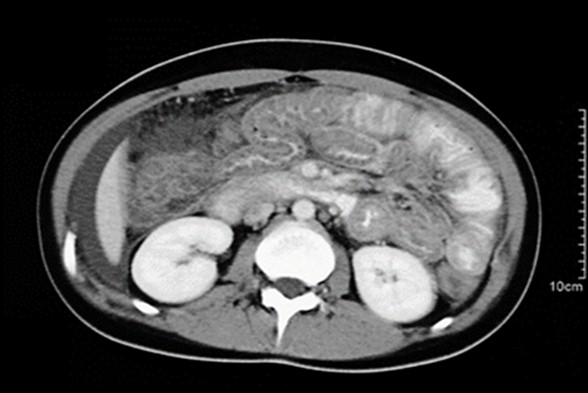
\includegraphics[width=10cm]{images/medicine/img9.jpg}
    \caption{Hình ảnh CT khoan bụng của một người trưởng thành \cite{ctimage}. }
\end{figure}

\subsubsection{Chất lượng ảnh CT thường được đánh giá bằng những tiêu chí sau:}
\paragraph{Độ phân giải không gian}là một thuật ngữ khác được sử dụng để phân giải chi tiết. Độ phân giải không gian là khả năng của hệ thống phân biệt được những hình dạng riêng biệt, những vật thể nhỏ nằm gần nhau. Độ phân giải không gian có thể được đo bằng hai phương pháp. Nó có thể được đo trực tiếp, hoặc có thể được tính từ phân tích sự lan truyền thông tin trong hệ thống.  Điều này phân tích dữ liệu sau được gọi là hàm truyền điều chế (MTF). Bằng cách định lượng độ phân giải không gian ở một trong những cách, có thể so sánh hiệu năng của hệ thống với hệ thống CT khác hoặc cùng hệ thống vào một ngày khác.
\vspace{-0.7cm}
\paragraph{Độ phân giải tương phản}là khả năng của hệ thống có thể phân biệt những vật thể có cùng mật độ trên hình ảnh. 

\subsection{Đơn vị Hounsfield}
Hounsfield unit đo mức độ hấp thụ tia X của một đối tượng. Trong X-quang thông thường, ta phải xác định trực quan những sắc thái của màu xám và phỏng đoán mật độ của những cấu trúc bên trong cơ thể bệnh nhân. Trong CT, chúng ta có thể định lượng khả năng làm suy giảm một chùm tia X của một đối tượng nhất định. Các phép đo được thể hiện bằng đơn vị Hounsfield (HU), được đặt theo tên của Godfrey Hounsfield, một trong những người tiên phong trong việc phát triển CT. Các đơn vị này cũng được gọi là số CT hoặc giá trị mật độ. Có thể hiểu HU là định lượng mức độ mà một cấu trúc làm suy giảm chùm tia X.\par

Hounsfield đã được gán nước cất với số 0, số 1000 cho xương và số $-1000$ cho không khí. Các vật thể có mức độ suy giảm chùm tia nhỏ hơn nước sẽ có giá trị Hounsfield âm, ngược lại sẽ có giá trị dương. Giá trị đơn vị của Hounsfield liên quan trực tiếp đến hệ số suy giảm tuyến tính: 1 HU bằng chênh lệch 0,1 phần trăm  giữa hệ số suy giảm tuyến tính của mô so với hệ số suy giảm tuyến tính của nước. Hệ số hấp thụ tuyến tính là lượng chùm tia x bị tán xạ hoặc bị hấp thụ trên một đơn vị độ dày của chất hấp thụ. 

\begin{figure}[H]
    \centering
    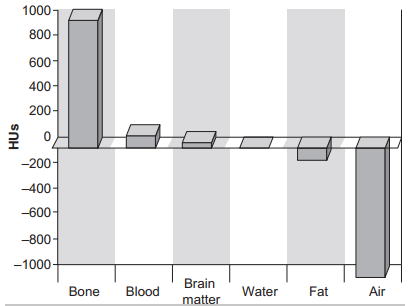
\includegraphics[width=12cm]{images/medicine/img2.png}
    \caption{Các đơn vị Hounsfield gần đúng \cite{ctimage}. }
\end{figure}
\vspace{-0.5cm}
Các ảnh CT tuân theo chuẩn DICOM (Digital Image and Communications in Medicine) thông thường sẽ có một kênh và được biểu thị bằng số nguyên 16-bit và được tổ chức xếp nhiều ảnh với nhau thành ảnh 3 chiều. Lúc này điểm ảnh pixel trên không gian hai chiều sẽ trở thành điểm ảnh voxel trên không gian ba chiều. Ảnh CT 3 chiều này sẽ đi kèm theo các thông tin về khoảng cách thực tế giữa hai voxel gần nhau trong không gian ba chiều. Nhờ đó ta có thể tính được diện tích và thể tích của vật thể nhờ vào số voxel của ảnh đó.\par

Mỗi lát cắt CT đại diện cho một vùng cụ thể trong cơ thể bệnh nhân. Độ dày của vùng này tương ứng với chiều dài theo trục Z. Dữ liệu thu thập từ máy CT được phân thành những phần tử: chiều dài đại diện bởi trục X, chiều cao đại diện bởi trục Y. Mỗi một hình vuông 2 chiều này là 1 pixel. Tập hợp hàng nghìn pixel tạo ra hình ảnh CT được hiển thị trên màn hình máy CT. Nếu mỗi pixel được bao gồm cả trục Z, thì lúc này pixe được gọi là voxel.
\begin{figure}[H]
    \centering
    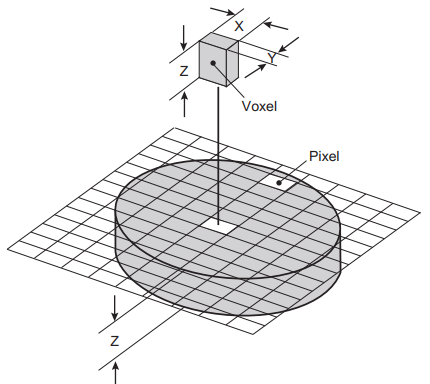
\includegraphics[width=8cm]{images/medicine/img1.png}
    \caption{Dữ liệu hình thành lát cắt CT được chia thành các phần tử \cite{ctimage}.} 
\end{figure}

% \subsection{Các loại dữ liệu}
% \subsubsection{Dữ liệu thô}
% Hàng ngàn bit dữ liệu thu thập được từ hệ thống gọi là dữ liệu thô. Quá trình sử dụng dữ liệu thô để tái tạo hình ảnh gọi là quá trình dựng ảnh. Việc xây dựng ảnh được tự động tạo ra trong quá trình quét thường được gọi là tái thiết trong tương lai (prospective reconstruction). Dữ liệu thô tương tự có thể được sử dụng sau này để tạo ra một hình ảnh mới. Quá trình này được gọi là tái thiết hồi cứu (retrospective reconstruction). Bởi vì dữ liệu thô bao gồm tất cả các phép đo thu được từ máy quét, nhiều hình ảnh có thể được tạo từ cùng một dữ liệu.
% \vspace{-0.5cm}
% \subsubsection{Dữ liệu hình ảnh}
% Để tạo thành một hình ảnh, máy tính gán một giá trị (đơn vị Hounsfield) cho mỗi pixel). Giá trị này (số mật độ), là trung bình của tất cả các phép đo suy giảm cho pixel đó. Pixel hai chiều đại diện cho một phần ba chiều của mô bệnh nhân. Giá trị pixel đại diện cho tỷ lệ  lượng năng lượng tia X đi qua mô và đến máy thu. Khi dữ liệu được tính trung bình để mỗi pixel có một số cụ thể, một hình ảnh có thể được hình thành. Dữ liệu trong hình ảnh này gọi là dữ liệu hình ảnh. Dữ liệu hình ảnh đòi hỏi khoảng 1/5 dung lượng bộ nhớ so với dữ liệu thô. Dữ liệu hình ảnh cho phép các phép đo như đơn vị Hounsfield, độ lệch chuẩn, khoảng cách nhưng không thể phân tích những thứ không quan sát được trên hình ảnh. Tóm lại, một giá trị đơn vị Hounsfield sẽ được gán cho một pixel. 

\section{Kỹ thuật phân đoạn ảnh}
\subsection{Định nghĩa}
Trong lĩnh vực xử lý ảnh, kỹ thuật phân đoạn ảnh (image segmentation) hay còn gọi pixed-level classification thực hiện nhiệm vụ phân vùng các đối tượng trong ảnh thành tập hợp các pixel. Điều đó có nghĩa là chúng ta cần phân biệt được các đối tượng quan tâm (gan, mạch máu,...) và phần còn lại của ảnh (nền ảnh). \par

Một cách hiểu khác, nhiệm vụ của nó là ta xác định trong có cái gì trong hình này, và nó nằm ở đâu trong ảnh. \par

Cụ thể hơn, mục đích của phân đoạn ảnh là gắn nhãn cho từng pixel (voxel cho ảnh 3D). Bởi vì việc dự đoán lớp của từng pixel trong ảnh nên nó còn có một tên khác dense prediction.

\begin{itemize}
    \item[] Kỹ thuật phân đoạn ảnh mang lại nhiều hiệu quả trong nhiều lĩnh vực:
	\item Phát triển xe tự hành (autonomous vehicles) như việc nhận diện các biển báo, người qua đường, phát hiện đèn dừng xe,... 
	\item Hình ảnh y tế: phát hiện khối u trong não, gan,... xây dựng lại hệ thống mạch máu, hiển thị một cách trực quan các bộ phận bên trong cơ thể. Từ đó hỗ trợ các bác sĩ đưa ra chuẩn đoán chính xác hơn, chuẩn bị chiến lược cần thiết trước quá trình phẫu thuật.
	\item Một số ứng dụng nhận dạng khác như: nhận dạng vân tay, khuôn mặt, võng mạc,...
\end{itemize}

\subsection{Hướng tiếp cận phân đoạn ảnh}
\subsubsection{Phân đoạn dựa theo ngưỡng}
Là thuật toán phân đoạn đơn giản nhất. Phương pháp phân đoạn theo ngưỡng dựa trên những giá trị cường độ của các điểm ảnh và những điểm lân cận với nó liệu có lớn hơn hay nhỏ hơn một ngưỡng đang xét để phân loại pixel đó thuộc lớp nào.

\newpage
% Để việc phân đoạn theo ngưỡng đạt kết quả cao, việc chọn ngưỡng cho phù hợp là bài toán máy tính cần xử lý một cách tự động. Do đó có sự xuất hiện của nhiều thuật toán có thể kể đến như: 
% \begin{itemize}
% 	\item Phương pháp dựa trên cụm (Clustering-based methods).
% 	\item Phương pháp dựa trên lược đồ Histogram (Histogram shape-based methods).
% 	\item Phương pháp dựa trên thuộc tính đối tượng (Object Attribute-based methods).
% 	\item Phương pháp dựa trên Entropy (Entropy-based methods).
% 	\item Phương pháp không gian (Spatial methods).
% 	\item Phương pháp dựa trên tính chất cục bộ (Local method).
% \end{itemize}

\subsubsection{Phân đoạn dựa theo miền đồng nhất}
Là kỹ thuật phân đoạn ảnh dựa trên yếu tố về không gian, màu sắc để ước lượng tính đồng nhất của miền. Việc lựa chọn các tính chất để phân vùng sẽ xác định tiêu chuẩn của vùng đó.
Các phương pháp có thể kể đến như:
\begin{itemize}
	\item Phương pháp tách cây tứ phân.
	\item Phương pháp phân vùng hợp.
	\item Phương pháp tách hợp (split-merge).
\end{itemize}

\subsubsection{Phân đoạn dựa trên mô hình mạng học sâu (Deep Learning)}
Các kỹ thuật phân đoạn truyền thống kể trên phần nào giải quyết được bài toán nhưng độ chính xác chưa cao, dễ bị sai khi bức ảnh không có sự rõ ràng màu sắc, độ tương quan... giữa các đối tượng.\par 

Hiện nay, với sự phát triển của mô hình mạng học sâu và sự tiến bộ về phần cứng đã đưa các giải pháp học máy hứa hẹn hơn, độ chính xác của mô hình đã tăng một cách đáng kể so với các phương pháp truyền thống. Trong các cuộc thi xử lý ảnh gần đây, các phương pháp dựa trên mạng học sâu luôn giành kết quả đứng đầu ở hầu hết các bài toán không chỉ xử lý ảnh mà còn cả xử lý ngôn ngữ tự nhiên, xử lý tín hiệu. Chi tiết ta có thể tham khảo thêm tại bài báo đánh giá các phương pháp mô hình học sâu trên ảnh y khoa tại đây \cite{reviewDLmedical}.

\section{Mạng học sâu}
Học sâu (Deep learning) là một kĩ thuật của máy học (Machine learning) dựa trên một tập hợp các thuật toán với mục tiêu mô hình dữ liệu trừu tượng thông qua nhiều lớp xử lý phức tạp (nhiều lớp biến đổi phi tuyến).\par

Một trong những phương pháp học sâu thành công nhất là mạng nơ-ron nhân tạo (Artificial Neural Network) hay cao hơn là Deep Neural Network được đề xuất bởi 2 người đoạt giải Nobel David H. Hubel và Torsten Wiesel. \par

Mạng nơron nhân tạo là một mô hình toán học (hay mô hình tính toán) được xây dựng dựa trên ý tưởng của mạng nơ-ron sinh học, bao gồm có một nhóm các nơ-ron nhân tạo (unit) nối với nhau và xử lý thông tin bằng cách truyền theo các kết nối và tính giá trị mới tại các nút. Trong nhiều trường hợp, mạng nơ-ron nhân tạo là một hệ thống thích ứng (adaptive system) tự thay đổi cấu trúc của mình dựa trên các thông tin bên ngoài hay bên trong chảy qua mạng trong quá trình học. \par

Mạng nơ-ron giống như bộ não con người, được học bởi kinh nghiệm (thông qua huấn luyện), có khả năng lưu giữ những kinh nghiệm tri thức và sử dụng những tri thức đó trong việc dự đoán các dữ liệu chưa biết (unseen data). Kiến trúc chung của một mạng nơron nhân tạo gồm 3 thành phần đó là: lớp đầu vào (input layer), lớp ẩn (hidden layer) và lớp đầu ra (output layer). 

\subsection{Thách thức đối với mạng học sâu}
Một mô hình học sâu đủ lớn có thể mô hình hóa bất kì mối quan hệ nào của dữ liệu. Tuy nhiên để huấn luyện được nó là một thách thức lớn, nhiều vấn đề có thể nảy sinh trong quá trình huấn luyện như tình trạng quá khớp (overfitting) hay thời gian tính toán quá dài, có khả năng không hội tụ tại nghiệm tối ưu. \par

Các mô hình có thiên hướng xảy ra hiện tượng quá khớp vì được thêm các lớp trừu tượng, mà cho phép chúng thực hiện mô hình hóa phụ thuộc vào các ngoại lệ của dữ liệu huấn luyện. Để tránh overfitting, có rất nhiều kỹ thuật được sử dụng, điển hình là cross-validation và regularization. Ngoài ra còn một phương pháp khác gần đây được áp dụng rất phổ biến dropout regularization. Dropout là một phương pháp tắt ngẫu nhiên các unit trong mô hình mạng. Điều này không những giúp phá vỡ các phụ thuộc từ các ngoại lệ của dữ liệu có thể xảy ra mà còn giúp lượng tính toán giảm đi đáng kể.

\subsection{Ứng dụng mạng học sâu trong phân đoạn ảnh}
Một hướng tiếp cận phổ biến trong bài toán phân đoạn ảnh dựa trên mạng học sâu là xây dựng mô hình theo kiến trúc Encoder-Decoder. Có nghĩa là, kiến trúc tổng thể của ta gồm 2 phần chủ yếu, một phần đại diện cho việc mã hóa đặc trưng dữ liệu có ích (có ý nghĩa cho việc phân loại từng pixel), phần còn lại tái cấu trúc (khôi phục) bản đồ đặc trưng tương ứng với ảnh đầu vào ban đầu. \par

Một số kiến trúc mạng được sử dụng cho bài toán phân đoạn ảnh phổ biến như sau, chi tiết có thể kham khảo thêm tại bài báo gốc: 
\vspace{-0.5cm}
\begin{itemize}
    \item U-Net: Convolutional Networks for Biomedical Image Segmentation \cite{Unet}.
	\item Fully Convolutional Networks for Semantic Segmentation (FCN) \cite{FCN}.
	\item Mask R-CNN \cite{RCNN}.
\end{itemize}

\subsubsection{Một số lớp chính trong mạng học sâu}
\paragraph{Lớp tích chập}là lớp tính toán dùng để trích xuất các đăc trưng từ ảnh, từ đó có thể đưa ra giá trị dự báo phân lớp dựa trên các đặc trưng đã trích xuất được. Trong lớp tính toán tích chập chứa các tham số (kernel) đã được học để tự điều chỉnh lấy ra những thông tin chính xác nhất mà không cần chọn các đặc trưng cụ thể (feature).\par

Phép tích chập được thực hiện trên giá trị đầu vào của dữ liệu và kernel (filter) để tạo ra một bản đồ đặc trưng (feature map). Một mạng tích chập cần nhiều feature map, thực hiện tương tự quá trình tích chập cho từng đặc trưng khác nhau, kết quả thu được là một tập hợp các đặc trưng có ích, tương ứng với mỗi bộ lọc.\par

Về mặt toán học, tích chập của hàm số $f$ và $g$ được viết là $ (f\ast g)$ có thể thể hiện như sau:
\begin{equation}
	{(f*g)(t)\ \ } {\stackrel {\mathrm {def} }{=}} {\ \ \int_{-\infty }^{\infty }f(\tau )\,g(t-\tau ) d\tau}
\end{equation}

Trong đó f đại diện cho ảnh ban đầu, g là bộ lọc của phép tích chập (filter).

Bộ lọc (filters) có kích thước nhỏ hơn so với ảnh (thường ma trận 3x3 hoặc 5x5). Tiến hành tích chập, bộ lọc sẽ dịch chuyển trên ảnh theo bước trượt chạy dọc theo ảnh và quét toàn bộ ảnh thu được feature map. Để tính toán sự khớp của một đặc trưng đối với một hình ảnh, ta thực hiện nhân mỗi điểm ảnh trong feature với giá trị của điểm ảnh tương ứng trong hình ảnh và lấy tổng của chúng.

\begin{figure}[H]
	\begin{center}
		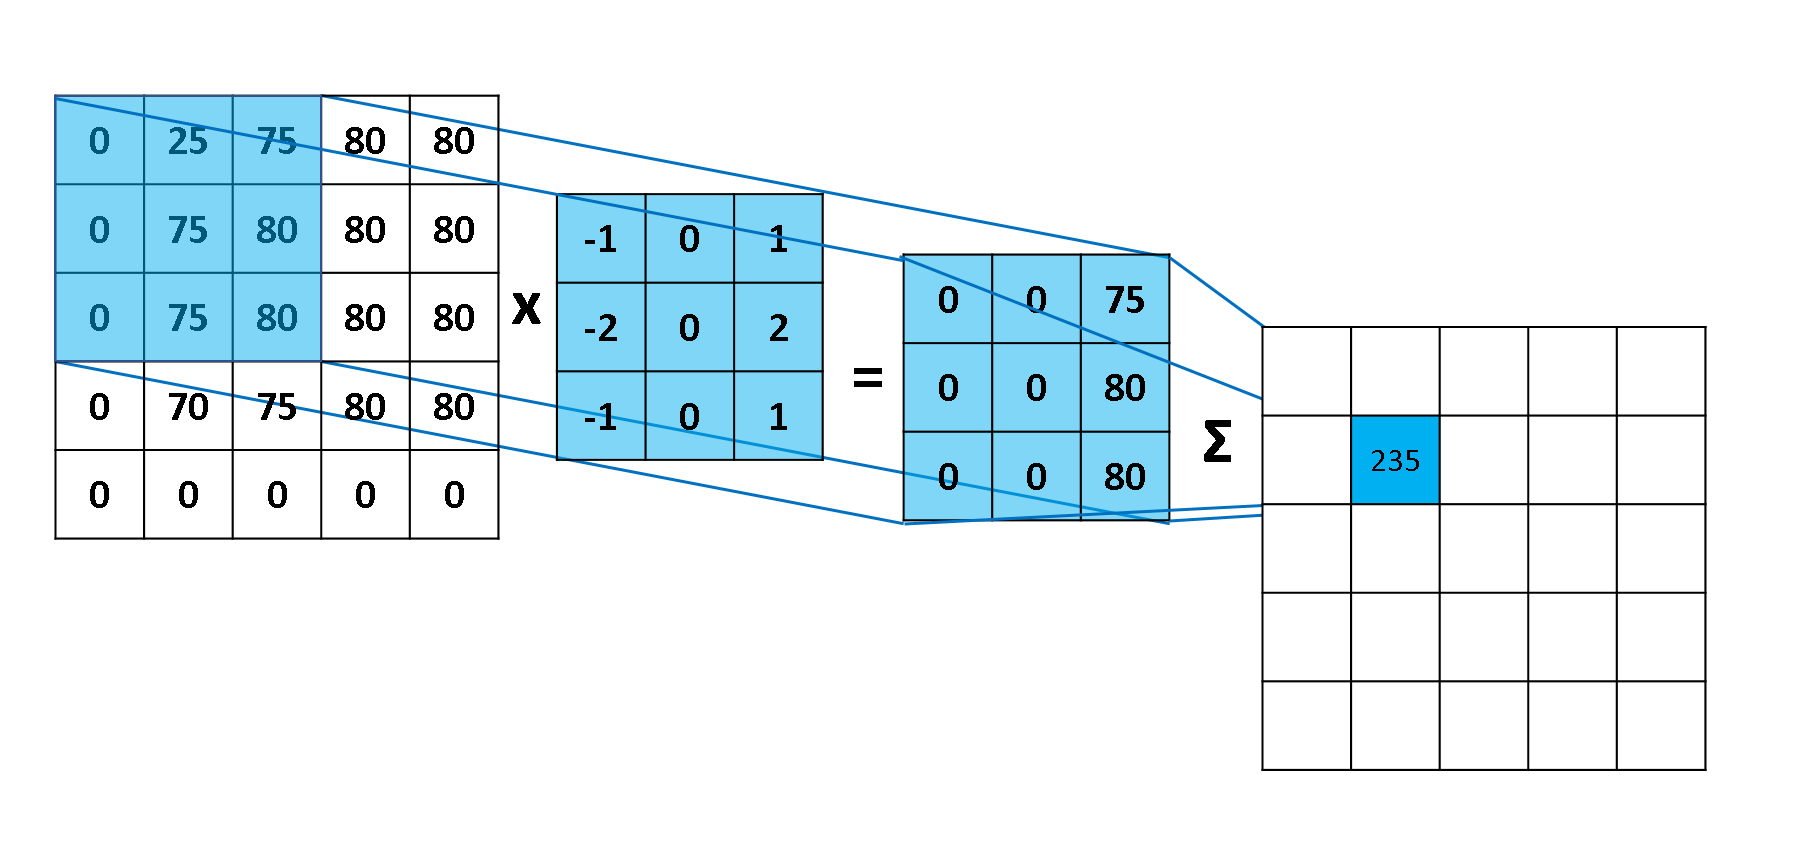
\includegraphics[width=12cm]{images/blood/convExample.png}
		\caption{Ví dụ minh họa về phép tích chập \cite{CNN}}
	\end{center}
\end{figure}

Thực hiện tương tự quá trình tích chập cho từng đặc trưng khác, kết quả thu được là một tập hợp các đặc trưng được trích xuất tương ứng với mỗi bộ lọc. 

Có hai dạng tính tích chập chính mà ta thường dùng là Valid và Same. Hai dạng cho ảnh kết quả có kích thước khác nhau:
\begin{itemize}
	\item Dạng Valid: kernel được trượt trên toàn ảnh, sau khi tính tích chập kết quả sẽ nhỏ hơn kích thước ảnh ban đầu. Với ảnh đầu vào có kích thước (m x m), kernel kích thước (n x n) thì ảnh đầu ra sẽ có kích thước (m-n+1)x(m-n+1). 
	\item Dạng Same: trước khi tính tích chập, ảnh sẽ được đệm (padding) thêm các giá trị (thường các giá trị này sẽ là 0 hoặc 1) để tăng kích thước ảnh, sao cho sau khi thực hiện Convolution, kích thước ảnh kết quả sẽ bằng với kích thước ảnh ban đầu.
\end{itemize}

\paragraph{Lớp gộp (Pooling layer)}có tác dụng giúp loại bỏ những thông tin không cần thiết, thường được sử dụng sau lớp tích chập. Rất hữu ích khi làm giảm độ phức tạp khi tính toán, tuy nhiên nếu lạm dụng nhiều có thể làm mất dữ liệu. \par

Trong lớp này sử dụng cửa sổ trượt, mỗi lần trượt theo một bước trượt (stride) cho trước. Khác với lớp tích chập, lớp gộp không tính tích chập mà tiến hành lấy mẫu (sub-sampling). Một giá trị đại diện thông tin ảnh tại vùng ảnh đó được giữ lại. Một số phương pháp phổ biến được sử dụng trong lớp gộp là max pooling (lấy giá trị lớn nhất), min pooling (lấy giá trị nhỏ nhất) và average pooling (lấy giá trị trung bình). \par

Ví dụ minh họa: mô hình có kích thước (4x4), lớp gộp dùng bộ lọc (2x2), bước trượt là 2, sử dụng phương pháp Max Pooling. Tiến hành gộp ảnh, giá trị lớn nhất trong vùng cửa sổ (2x2) giới hạn bởi bộ lọc được giữ lại, làm đầu ra. Sau lớp gộp, kích thước ảnh giảm đi 2 lần mỗi chiều (2x2). 

\begin{figure}[H]
	\begin{center}
		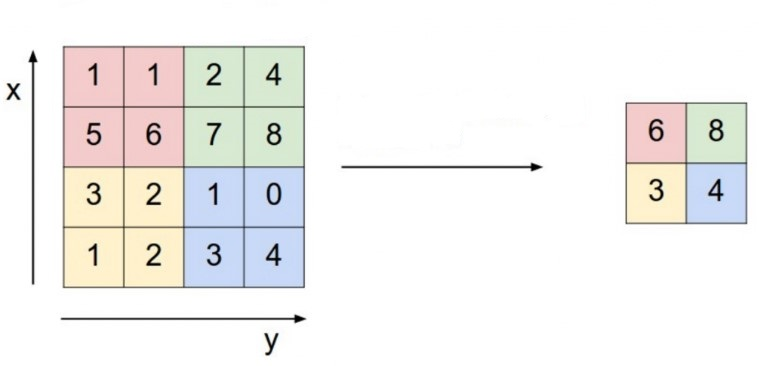
\includegraphics[width=12cm]{images/blood/maxpool.jpg}
		\caption{Minh họa lớp Max Pooling \cite{CNN}}
	\end{center}
\end{figure}

Khi dữ liệu ảnh có kích thước lớn, thực hiện qua nhiều lớp gộp sẽ thu nhỏ, giảm kích thước dữ liệu. Từ đó làm giảm lượng tham số, tăng hiệu quả tính toán và góp phần kiểm soát hiện tượng quá khớp (overfitting). \par

Ta có thể thấy, sau khi chạy qua các lớp gộp các đặc trưng khác nhau sẽ nằm gần lại với nhau hơn. Nhờ đó, lớp tích chập phía sau sẽ trích xuất được thông tin ở vùng lớn hơn vùng ở lớp đầu. Vì vậy, qua nhiều lớp gộp và tích chập, đặc trưng thu được sẽ có ý nghĩa toàn cục hơn là ý nghĩa chi tiết. \par

Lớp gộp sẽ cho bạn tính bất biến đối với phép dịch chuyển (translation), phép quay (rotation) và phép co giãn (scaling). Tính kết hợp cục bộ cho ta các cấp độ biểu diễn thông tin từ mức độ thấp đến mức độ cao và trừu tượng hơn thông qua lớp tích chập từ các bộ lọc.

%%%%%%%%%%%%%%% (start) metric to evaluate 
\newpage
\section{Các phương pháp đánh giá mô hình phân đoạn ảnh}\label{evaluation-methods}
Khi xây dựng một mô hình mạng học sâu, chúng ta cần một công cụ để có thể đánh giá xem mô hình có hoạt động hiệu quả hay không đồng thời giúp chúng ta đánh giá khả năng giữa các mô hình. \par

Hiệu năng của một mô hình được đánh giá trên tập dữ liệu kiểm thử (test dataset). Giả sử khi cho đầu vào chạy qua mô hình ta sẽ được đầu ra của tập kiểm thử là các dự đoán của mô hình (gọi là y predict). Đó là một bức ảnh dưới dạng tensor với những giá trị xác xuất dự đoán thuộc lớp nào. Còn y true đại diện cho tensor với nhãn thật của dữ liệu. Do đó ta cần so sánh giữa 2 tensor y predict và y true.\par

\subsection{Ma trận nhầm lẫn}
Khi đánh giá một mô hình mạng học sâu, chúng ta thường đề cập đến một thuật ngữ gọi là ma trận nhầm lẫn (\textbf{confusion matrix}) \cite{confution}. Một bảng dùng để mô tả hiệu suất của một mô hình phân loại trên tập dữ liệu đã biết kết quả đúng, giúp ta có cái nhìn trực quan về hiệu suất các giải thuật.
\begin{table}[H]
\centering
\begin{tabular}{l|l|c|c|}
	\multicolumn{2}{c}{}	&	\multicolumn{2}{c}{Giá trị thực}	\\
	\cline{3-4}
	\multicolumn{2}{c|}{}					   & Positive &	Negative \\
	\cline{2-4}
	\multirow{2}{*}{Giá trị dự đoán}& Positive & TP 	  & FP 		 \\
	\cline{2-4}
									& Negative & FN		  & TN	 	 \\
	\cline{2-4}
\end{tabular}
\caption{Ma trận nhầm lẫn}
\label{confution_matrix}
\end{table}
\vspace{-5mm}
Cụ thể hơn, khi xét một bài toán phân loại 2 lớp: trong đó một lớp nghiêm trọng hơn lớp kia cần được đự doán chính xác. Giả sử ta đang xét bài toán phân loại gồm 2 lớp: ung thư (positive), không ung thư (negative).
\begin{itemize}[noitemsep, topsep=0pt]
	\item Positive: Đối tượng được gán nhãn là ung thư.
	\item Negative: Đối tượng được gán nhãn là không phải ung thư.
	\item True Positive (TP): Khi mô hình dự đoán đúng đối tượng đó là ung thư.
	\item False Positive (FP): Khi mô hình dự đoán đối tượng đó là ung thư nhưng thực sự nó là không phải là ung thư.
	\item True Negative (TN): Khi mô hình dự đoán đúng đối tượng đó là không phải ung thư.
	\item False Negative (FN): Khi mô hình dự đoán đối tượng đó là không phải ung thư nhưng thực sự nó là ung thư.
\end{itemize}

Bên cạnh đó, các chỉ số False Positive Rate (tỉ lệ báo động nhầm), False Negative Rate (tỉ lệ bỏ sót) cũng đáng được quan tâm. 
\begin{equation}
	\mathrm{FPR} = \mathrm{\frac{FP}{FP + TN}} \hspace{0.5cm}
	\mathrm{FNR} = \mathrm{\frac{FN}{TP + FN}}
\end{equation} 

Ví dụ, trong bài toán xác định có bệnh ung thư hay không thì việc không bị sót quan trọng hơn là việc chẩn đoán nhầm âm tính thành dương tính. Hay trong bài toán lọc email rác thì việc cho nhầm email quan trọng vào thùng rác nghiêm trọng hơn việc xác định một email rác là email thường. \par

Với các bài toán có nhiều lớp dữ liệu, ta có thể xây dựng bảng True/False Positive/Negative cho mỗi lớp nếu coi lớp đó là lớp Positive, các lớp còn lại gộp chung thành lớp Negative.

% \subsection{Pixel Accuracy}
% Một cách đánh giá cơ bản cho bài toán phân đoạn ảnh là tính tỉ lệ pixels (voxel) của ảnh đó được phân loại đúng.
% Tuy nhiên trong bài toán phân đoạn (còn gọi dense prediction) đôi khi độ đo accuracy không thể hiện được mô hình liệu có hiệu suất tốt hay không vì xuất hiện các vấn đề như: mất cân bằng dữ liệu (một lớp trong ảnh có tỉ lệ xuất hiện quá nhỏ so với lớp còn lại). Miền giá trị của độ đo [0,1] (hay $0-100\%$).
% \begin{equation}
% \begin{aligned}
% 	\mathrm{accuracy} = \mathrm{\frac{TP + TN}{TP + TN + FP + FN}}
% \end{aligned}
% \end{equation}

\subsection{Độ chính xác và độ truy hồi }
Độ chính xác (precision) được định nghĩa là tỉ lệ số điểm được đánh giá là True Positive trong những điểm được phân loại là positive.
Độ truy hồi (recall) được định nghĩa là tỉ lệ số điểm được đánh giá là true positive trong số những điểm thực sự là positive. 

\begin{equation}
    \mathrm{Precision = \frac{TP}{TP + FP}} \hspace{0.5cm}
    \mathrm{Recall = \frac{TP}{TP + FN}}
\end{equation}

Xét trường hợp precision = 1, có nghĩa là mọi điểm tìm được đều thực sự là positive, tức không có điểm negative nào lẫn vào kết quả. Tuy nhiên vẫn chưa đủ khẳng định là mô hình thực sự tốt, vì nó không đánh giá những điểm positive thật sự đã được phân loại đủ hay chưa. Do đó,nếu một mô hình chỉ tìm được đúng một điểm positive mà nó chắc chắn nhất thì ta không thể gọi nó là một mô hình tốt.
\newpage
Xét trường hợp recall = 1, có nghĩa là mọi điểm positive đều được tìm thấy. Tuy nhiên, đại lượng này lại không đo liệu có bao nhiêu điểm negative bị lẫn trong đó. Nếu mô hình phân loại mọi điểm là positive thì chắc chắn recall = 1, tuy nhiên dễ nhận ra đây là một mô hình cho kết quả cực kì tệ.\par

Một mô hình phân loại tốt là mô hình có cả Precision và Recall đều cao, tức càng gần một càng tốt. Có hai cách đo chất lượng của bộ phân lớp dựa vào Precision và Reall: Precision-Recall curve và F1-score (Dice).
\vspace{-0.25cm}
% \subsection{Intersection over Union (IoU)}
% Độ đo IoU (hay được biết đến Jascard Index \cite{iou}) là một trong những độ đo được sử dụng phổ biến trong bài toán phân đoạn ảnh.\par 

% Ý tưởng cơ bản là IoU là tập hợp những pixel thuộc chung một lớp (phần trùng lắp) giữa giá trị phân đoạn do mô hình dự đoán và nhãn thực (ground truth) của nó. Độ đo này có phần gần giống với hệ số Dice, chúng thường được sử dụng trong hàm đánh giá mất mát trong quá trình huấn luyện. \par

% \begin{equation} 
% \begin{aligned}
% 	\mathrm{IoU} = \frac{|\mathrm{Predict} \cap \mathrm{Target}|}{|\mathrm{Predict} \cup \mathrm{Target}|}
% 				= \mathrm{\frac{TP}{TP + FP + FN}}
% \end{aligned}
% \end{equation}

% Đơn giản hơn, IoU tính số lượng pixel được dự đoán chung lớp của cả giá trị mục tiêu và dự đoán, giá trị này chia cho tổng số pixel được dự đoán là thuộc lớp đó của cả 2 giá trị mục tiêu và dự đoán.

\subsection{Hệ số tương đồng Dice}
Hệ số tương đồng Dice (hay còn gọi F1 Score) là một phương pháp thống kê dùng để đo độ giống nhau giữa hai mẫu được giới thiệu bởi Thorvald Sørensen\cite{dice1} và Lee Raymond Dice\cite{dice}. \par

Hệ số Dice ban đầu được phát triển cho dữ liệu 2 lớp. Có thể tính bằng cách lấy 2 lần khu vực trùng lắp lên nhau của giá trị dự đoán và nhãn thực chia cho tổng số pixel của ảnh. Độ đo có miền giá trị từ [0,1] với giá trị 1 thể hiện cho việc trùng lắp hoàn hảo giữa giá trị dự đoán và giá trị thực.
\begin{equation}
	\mathrm{Dice(A, B)} = \mathrm{\frac{2 * |A \cap B|}{|A| + |B|}}
\end{equation} 

Trong đó, A là một ảnh đầu ra của mô hình, chứa các giá trị xác xuất do mô hình dự đoán có thể đúng hoặc sai. B là một ảnh (gọi là ảnh mục tiêu) chứa tập hợp những giá trị cho từng pixel được gán nhãn bởi chuyên gia. A và B có cùng kích thước. $|\mathrm{A}|$ đại diện cho toàn bộ pixel thuộc ảnh A. \par 

Có thể hiểu đơn giản, $|\mathrm{A} \cap \mathrm{B}|$ đại diện cho tập hợp những pixel thuộc cùng một lớp của tập A và B. 

\hspace{-2.0cm}
\begin{tabular}{c c c c c}
	$\left[
	\begin{matrix}
		0.19 & 0.65 & 0.11 & 0.04\\
		0.55 & 0.55 & 0.67 & 0.12\\
		0.01 & 0.16 & 0.05 & 0.11\\
		0.72 & 0.91 & 0.67 & 0.99
	\end{matrix}
	\right]$ & $*$ &
	$\left[
	\begin{matrix}
		0 & 0 & 0 & 0\\
		1 & 1 & 1 & 1\\
		1 & 1 & 1 & 1\\
		0 & 0 & 0 & 0
	\end{matrix}
	\right]$ & $ \underrightarrow{\mathrm{element-wise}}$ &
	$\left[
	\begin{matrix}
		0	 & 0 	& 0 	& 0\\
		0.55 & 0.55 & 0.67 	& 0.12\\
		0.01 & 0.16 & 0.05 	& 0.11\\
		0 	 & 0 	& 0 	& 0
	\end{matrix}
	\right]$ \\ 
	Prediction &  & Target & sum   & \\
	& & & $ \myarrow[2.6cm] $ & $2.22$ 
\end{tabular}

Để định lượng cho giá trị $|\mathrm{A}|$ và $|\mathrm{B}|$, thông thường một số người chọn việc sử dụng tổng bên cạnh đó một số người lại sử dụng tổng bình phương để tính. Vậy nên cách tốt nhất để biết được nên định lượng bằng cách nào là tốt nhất ta nên thử nghiệm cả hai phương pháp tùy vào nhiệm vụ khác nhau sẽ đem lại kết quả tối ưu khác nhau.

\hspace{1.5cm}
\begin{tabular}{c c c}
	$|\mathrm{A}|$ =& 
	$\left[
	\begin{matrix}
		0.19 & 0.65 & 0.11 & 0.04\\
		0.55 & 0.55 & 0.67 & 0.12\\
		0.01 & 0.16 & 0.05 & 0.11\\
		0.72 & 0.91 & 0.67 & 0.99
	\end{matrix}
	\right]^{2 (optional)}$ & $\underrightarrow{\mathrm{sum}}$ 6.5\\ 
	$|\mathrm{B}|$ =&
	$\left[
	\begin{matrix}
	0 & 0 & 0 & 0\\
	1 & 1 & 1 & 1\\
	1 & 1 & 1 & 1\\
	0 & 0 & 0 & 0
	\end{matrix}
	\right]^{2 (optional)}$ & $\underrightarrow{\mathrm{sum}}$ 8
\end{tabular}

Một cách thể hiện khác dựa trên ma trận nhầm lẫn để tính hệ số Dice theo công thức sau:
\begin{equation}
	\mathrm{Dice} = \mathrm{\frac{2TP}{2TP + FP + FN}}
\end{equation}

\subsection{Chỉ số lỗi trùng thể tích}
Chỉ số lỗi trùng thể tích (Volumetric Overlap Error), được tính bằng cách lấy tổng số voxel giao giữa dự đoán và nhãn chia cho tổng số voxel hợp giữa dự đoán và nhãn, lấy 1 trừ kết quả đó ta được giá trị VOE.
\begin{align}
    % VOE = (1 - \frac{|\mathrm{Predict} \cap \mathrm{Target}|}{|\mathrm{Predict} \cup \mathrm{Target}|})*100\%
    \mathrm{VOE} &= 1 - \mathrm{\dfrac{TP}{TP + FN + FP}}
\end{align}

Với TP là số lượng điểm ảnh True Positive, FN là số lượng điểm ảnh False Negative và FP là số lượng điểm ảnh False Positive. Giá trị này là 0 khi phân đoạn hoàn hảo và là 1 (giá trị thấp nhất) khi không có sự chồng chéo nào giữa dự đoán và nhãn.

\subsection{Chỉ số sai khác thể tích}
Chỉ số sai khác thể tích (Volume Difference - VD), đơn vị phần trăm, được tính bằng hiệu số số voxel của dự đoán và nhãn, chia cho số voxel của nhãn..
\begin{align}
    % VD = (\frac{|\mathrm{Predict}| - |\mathrm{Target}|}{|\mathrm{Target}|})*100\%
    \mathrm{VD} &= \mathrm{\dfrac{FP - FN}{TP + FN}}
\end{align}
Với TP là số lượng điểm ảnh True Positive, FN là số lượng điểm ảnh False Negative và FP là số lượng điểm ảnh False Positive. Chỉ số này nhận giá trị âm khi thể tích phân đoạn nhỏ hơn thể tích nhãn và nhận giá trị dương khi thể tích phân đoạn lớn hơn thể tích nhãn.
